\documentclass[xcolor={dvipsnames,table}]{beamer}
\usepackage{epsfig,graphicx}
\usepackage{palatino}
\usepackage{fancybox}
\usepackage{relsize}
\usepackage[procnames]{listings}
\usepackage{hyperref}
\usepackage{qtree} % needed?
\usepackage{booktabs}
\usepackage{dirtree}
\usepackage[normalem]{ulem}
\usepackage{tikz}
\usetikzlibrary{arrows.meta,positioning,calc,fit,shapes.geometric,decorations.pathreplacing}


% fatter TT font
\renewcommand*\ttdefault{txtt}
% another TT, suggested by Alex
% \usepackage{inconsolata}
% \usepackage[T1]{fontenc} % needed as well?


\newcommand{\scale}{0.7}

\newcommand{\todo}[1]{{\emph{TODO: #1}}}
\newcommand{\martin}[1]{{\color{blue} Martin: #1}}
\newcommand{\abcdef}[1]{{\color{red} Author2: #1}}

% uncomment following for final submission
%\renewcommand{\todo}[1]{}
%\renewcommand{\martin}[1]{}
%\renewcommand{\author2}[1]{}

\newcommand{\code}[1]{{\texttt{#1}}}

\hypersetup{
  linkcolor  = black,
%  citecolor  = blue,
  urlcolor   = blue,
  colorlinks = true,
}

\beamertemplatenavigationsymbolsempty
\setbeamertemplate{footline}[frame number]




\newif\ifbook
% shared in slides and book

\lstdefinelanguage{chisel}{
  morekeywords={abstract,case,catch,class,def,%
    do,else,extends,false,final,finally,%
    for,if,implicit,import,match,mixin,%
    new,null,object,override,package,%
    private,protected,requires,return,sealed,%
    super,this,throw,trait,true,try,%
    type,val,var,while,with,yield},
  otherkeywords={=>,<-,<\%,<:,>:,\#,@},
  sensitive=true,
  morecomment=[l]{//},
  morecomment=[n]{/*}{*/},
  morestring=[b]",
  morestring=[b]',
  morestring=[b]"""
}

\usepackage{color}
\definecolor{dkgreen}{rgb}{0,0.6,0}
\definecolor{gray}{rgb}{0.5,0.5,0.5}
\definecolor{mauve}{rgb}{0.58,0,0.82}

% Default settings for code listings
\lstset{%frame=lines,
  language=chisel,
  aboveskip=3mm,
  belowskip=3mm,
  showstringspaces=false,
  columns=fixed, % basewidth=\mybasewidth,
  basicstyle={\small\ttfamily},
  numbers=none,
  numberstyle=\footnotesize\color{gray},
  % identifierstyle=\color{red},
  keywordstyle=\color{blue},
  commentstyle=\color{dkgreen},
  stringstyle=\color{mauve},
  breaklines=true,
  breakatwhitespace=true,
  procnamekeys={def, val, var, class, trait, object, extends},
  procnamestyle=\ttfamily\color{red},
  tabsize=2,
  float
}

\lstnewenvironment{chisel}[1][]
{\lstset{language=chisel,#1}}
{}

\newcommand{\shortlist}[1]{{\lstinputlisting[nolol]{#1}}}

\newcommand{\longlist}[3]{{\lstinputlisting[float, caption={#2}, label={#3}, frame=tb, captionpos=b]{#1}}}


\title{Generators for Design Space Exploration}
\author{Martin Schoeberl}
\date{3 November 2026}
\institute{Technical University of Denmark\\
Embedded Systems Engineering}
\begin{document}
\begin{frame}
\titlepage
\end{frame}
\begin{frame}{Organization}
\begin{itemize}
\item You have presented your MVP
\item What should you improve next?
\item Today: measure different generated designs
\item Standup presentations:
\begin{itemize}
\item 3 minutes per group, no slides
\item What did you last week?
\item What are your parameters?
\end{itemize}
\end{itemize}
\end{frame}

\begin{frame}{Outline}
\begin{itemize}
\item From generators to design space exploration (DSE)
\item Revisit our MaxFinder example
\item Measure area and timing with LibreLane
\item Estimated fmax, latency, and throughput
\item Use the results to plan the next sprint
\end{itemize}
\end{frame}

\begin{frame}{Why Generators for DSE?}
\begin{itemize}
\item One program generates many circuit variations
\item We can change the architecture with a parameter
\item Test all generated variants
\item Measure their implementation cost
\item Select a variant that meets our requirements
\item What does \emph{best} mean for your project?
\end{itemize}
\end{frame}

\begin{frame}{Remember MaxFinder?}
\begin{itemize}
\item Find the maximum of a vector of unsigned values
\item We used a tree reduction in lab 2
\item Keep the function fixed: 8 inputs, each 16 bits
\item Exact maximum, no approximation
\item A new input vector can arrive every cycle
\item Can we trade area for speed?
\end{itemize}
\end{frame}

\begin{frame}{What Do We Change?}
\begin{itemize}
\item Architecture: chain, tree, or pipelined tree
\item One clock target: 20 ns (50 MHz)
\item One YAML configuration for all three designs
\item Keep the cell library and synthesis strategy fixed
\item Compare the estimated maximum clock frequency
\item Changing the bit width also changes the problem!
\end{itemize}
\end{frame}


\begin{frame}{A Chain of Comparators}

\begin{center}
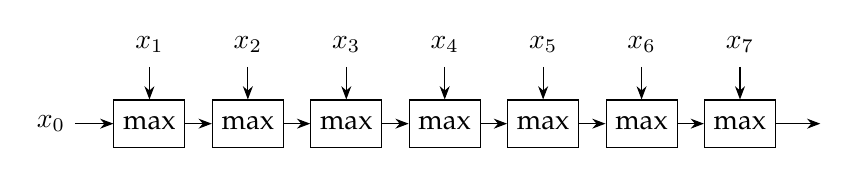
\begin{tikzpicture}[x=1.25cm,y=1cm,>=Stealth,
 m/.style={draw,minimum width=0.8cm,minimum height=0.6cm}]
\foreach \i in {1,...,7} {
 \node[m] (m\i) at (\i,0) {max};
 \node at (\i,1) {$x_{\i}$};
 \draw[->] (\i,0.72) -- (m\i.north);
}
\node (x) at (0,0) {$x_0$};
\draw[->] (x) -- (m1);
\foreach \i/\j in {1/2,2/3,3/4,4/5,5/6,6/7}
 \draw[->] (m\i) -- (m\j);
\draw[->] (m7.east) -- ++(0.45,0);
\end{tikzpicture}
\end{center}
\begin{itemize}
\item 7 compare/select operations
\item Up to 7 operations on one combinational path
\item Input and output registers are not shown
\item What happens when we double the input count?
\end{itemize}
\end{frame}

\begin{frame}{A Balanced Tree}

\begin{center}
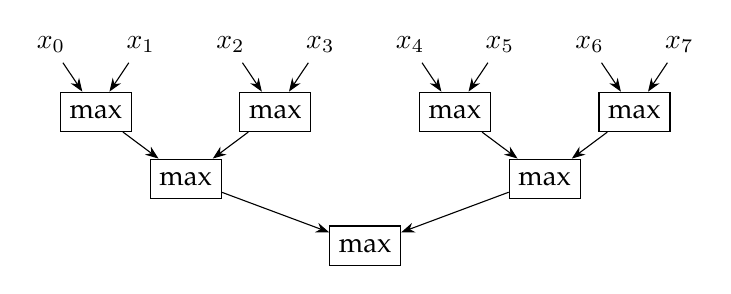
\begin{tikzpicture}[x=0.95cm,y=0.85cm,>=Stealth,
 m/.style={draw,minimum width=0.9cm,minimum height=0.5cm}]
\foreach \i/\x in {0/-4.2,1/-3,2/-1.8,3/-0.6,4/0.6,5/1.8,6/3,7/4.2}
 \node (x\i) at (\x,0) {$x_{\i}$};
\foreach \i/\x in {0/-3.6,1/-1.2,2/1.2,3/3.6}
 \node[m] (a\i) at (\x,-1) {max};
\foreach \i/\j in {0/0,1/0,2/1,3/1,4/2,5/2,6/3,7/3}
 \draw[->] (x\i) -- (a\j);
\node[m] (b0) at (-2.4,-2) {max};
\node[m] (b1) at (2.4,-2) {max};
\foreach \i/\j in {0/0,1/0,2/1,3/1}
 \draw[->] (a\i) -- (b\j);
\node[m] (c) at (0,-3) {max};
\draw[->] (b0) -- (c);
\draw[->] (b1) -- (c);
\end{tikzpicture}
\end{center}
\begin{itemize}
\item Still 7 operations, but only 3 levels
\item Input and output registers are not shown
\end{itemize}
\end{frame}

\begin{frame}{Pipeline the Tree}

\begin{center}
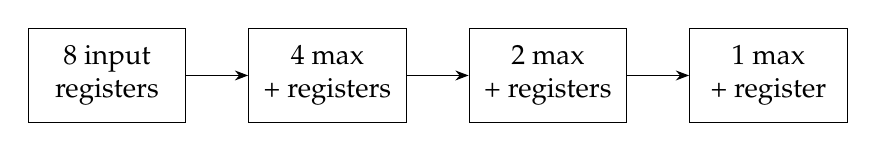
\begin{tikzpicture}[>=Stealth,
 s/.style={draw,align=center,minimum height=1.2cm,minimum width=2cm}]
\node[s] (a) at (0,0) {8 input\\registers};
\node[s] (b) at (2.8,0) {4 max\\+ registers};
\node[s] (c) at (5.6,0) {2 max\\+ registers};
\node[s] (d) at (8.4,0) {1 max\\+ register};
\draw[->] (a) -- (b);
\draw[->] (b) -- (c);
\draw[->] (c) -- (d);
\end{tikzpicture}
\end{center}
\begin{itemize}
\item One compare/select level between registers
\item More registers and more clock load
\item A new vector can still arrive every cycle
\item The result takes more cycles to arrive
\item Is this always an improvement?
\end{itemize}
\end{frame}

\begin{frame}{Predict Before Running}
\begin{itemize}
\item Which architecture has the smallest area?
\item Which one can run at the highest clock frequency?
\item Which one has the lowest transaction latency?
\item Discuss with your neighbor
\item Synthesis may restructure our circuit
\item Our RTL structure is a hypothesis, not a measurement
\end{itemize}
\end{frame}

\begin{frame}[fragile]{Generate the Chain}

\begin{chisel}
def maximum(a: UInt, b: UInt): UInt =
  Mux(a > b, a, b)

val inputs = VecInit(io.in.map(x => RegNext(x)))
io.out := RegNext(inputs.reduceLeft(maximum))
\end{chisel}
\begin{itemize}
\item Scala builds the chain during elaboration
\item Input and output are registered
\item A new input vector on every clock edge
\end{itemize}
\end{frame}

\begin{frame}[fragile]{Generate the Trees with reduceTree}
\begin{chisel}
// Balanced tree, with an output register
io.out := RegNext(inputs.reduceTree(maximum))

// Pipelined tree: register each compare/select
io.out := inputs.reduceTree(
  (a, b) => RegNext(maximum(a, b)))
\end{chisel}
\begin{itemize}
\item Two alternative implementations
\item \code{inputs} is a Chisel \code{Vec}, not a Scala sequence
\item Power-of-two input count: equal pipeline depth
\item No control signals: just a data pipeline
\end{itemize}
\end{frame}



\begin{frame}{What Is LibreLane?}
\begin{itemize}
\item An open-source flow from RTL to chip layout
\item Yosys maps our RTL to standard cells
\item Static timing analysis checks the clock target
\item OpenROAD handles physical implementation
\item Today we stop after synthesis and pre-PnR timing
\item Run the full flow later for selected candidates
\end{itemize}
\end{frame}

\begin{frame}[fragile]{One Configuration for All Three Designs}
\begin{lstlisting}[language={}]
DESIGN_NAME: MaxFinder
VERILOG_FILES:
  - dir::MaxFinder.sv
CLOCK_PORT: clock
CLOCK_PERIOD: 20
PDK: sky130A
STD_CELL_LIBRARY: sky130_fd_sc_hd
SYNTH_STRATEGY: AREA 0
\end{lstlisting}
\begin{itemize}
\item The Makefile selects the generated RTL directory
\item Same clock, IO assumptions, and timing corners
\end{itemize}
\end{frame}


\begin{frame}[fragile]{Let Us Run the Experiment}
\begin{lstlisting}[language={}]
sbt test
make generate

# Inside the LibreLane environment
make chain
make tree
make pipeline
make reports
\end{lstlisting}
\begin{itemize}
\item Run \code{make generate} before the LibreLane targets
\item Stop after synthesis and pre-PnR timing
\item Open the reports and inspect the critical path
\end{itemize}
\end{frame}


\begin{frame}{Which Metrics?}
\begin{itemize}
\item Cell area: sum of mapped standard-cell areas
\item This is not the die area
\item Setup slack = required time $-$ arrival time
\item Negative slack: the clock target is not met
\item Check the constraints and analyzed corners
\item Exclude failed or incomplete runs from the frontier
\end{itemize}
\end{frame}

\begin{frame}{Latency and Throughput}
\begin{itemize}
\item All three designs accept one vector per cycle
\item At 20 ns: 50 million vectors/s, if timing passes
\item Input is accepted at clock edge $k$
\item Chain/tree output appears after edge $k+1$
\item Pipelined tree output appears after edge $k+3$
\item Acceptance-to-output latency: 20 ns versus 60 ns
\item A downstream register captures one edge later
\end{itemize}
\end{frame}




\begin{frame}[fragile]{Find the Cell Area Estimate}
\begin{lstlisting}[language={}]
# From the dse directory, after make tree
cd build/rtl/tree/runs/timing
grep 'design__instance__area' final/metrics.json
\end{lstlisting}
\begin{itemize}
\item Mapped standard-cell area in $\mu$m$^2$
\item Repeat for \code{chain} and \code{pipeline}
\item Also in \code{*-yosys-synthesis/yosys-synthesis.log}
\item Search for \code{Chip area for module}
\item Use the final top-module result, not an earlier statistic
\item This is cell area, not floorplan or die area
\end{itemize}
\end{frame}

\begin{frame}[fragile]{Read the Clock Report}
\begin{lstlisting}[language={}]
# From build/rtl/tree/runs/timing
cd *-openroad-staprepnr
less nom_ss_100C_1v60/clock.rpt
\end{lstlisting}
\begin{itemize}
\item Search for \code{report\_clock\_min\_period}
\item Find \code{period\_min} (ns) and \code{fmax} (MHz)
\item $f_{max} \approx 1000 / T_{min}$
\item Compare the lowest fmax across all corner directories
\item Open that corner's \code{max.rpt}: what sets the limit?
\item Use \code{summary.rpt} to inspect the other checks
\end{itemize}
\end{frame}

\begin{frame}{Let Us Explore the Reports}
\begin{center}
\begin{tabular}{lrrr}
\toprule
Design & Cell area & Min. period & Est. fmax\\
 & $\mu$m$^2$ & ns & MHz\\
\midrule
Chain & ? & ? & ?\\[1ex]
Tree & ? & ? & ?\\[1ex]
Pipeline & ? & ? & ?\\
\bottomrule
\end{tabular}
\end{center}
\begin{itemize}
\item Fill in the table before we reveal the results
\item Use the same corner when comparing architectures
\item Which designs meet 50 MHz? What is the area cost?
\item Can you explain one critical path?
\end{itemize}
\end{frame}

\begin{frame}{Measured Area and Estimated fmax}
\begin{center}
\small
\begin{tabular}{lrrr}
\toprule
Design & Cell area & Min. period & Est. fmax\\
 & $\mu$m$^2$ & ns & MHz\\
\midrule
Chain & 7729 & 30.66 & 32.62\\
Tree & 7599 & 15.48 & 64.58\\
Pipeline & 8996 & 6.11 & 163.69\\
\bottomrule
\end{tabular}
\end{center}
\begin{itemize}
\item All runs use a 20 ns clock target
\item Slow-corner clock report, before placement/routing
\item LibreLane 3.0.3, SKY130A; 28 October 2026
\item Which designs meet our 50 MHz target?
\end{itemize}
\end{frame}


\begin{frame}{Which Architecture Would You Choose?}
\begin{itemize}
\item At 50 MHz, tree and pipeline have equal throughput
\item Tree: fewer cells and lower transaction latency
\item Pipeline: potential for a higher clock
\item About 18\% more cell area for that headroom
\item A point dominates another if no objective is worse
      and at least one is better
\item What changes when the throughput requirement rises?
\end{itemize}
\end{frame}



\begin{frame}{What Have We Not Measured Yet?}
\begin{itemize}
\item Placement, routing, and clock-tree effects
\item Timing with extracted wire parasitics
\item Physical checks: DRC and LVS
\item Power needs a workload and switching activity
\item Run full physical implementation for finalists
\item Do not mix early estimates and routed results
\end{itemize}
\end{frame}

\begin{frame}{Keep the Experiment Reproducible}
\begin{itemize}
\item Record generator parameters and generated RTL
\item Save the configuration, tool and PDK versions
\item Keep raw metrics and failed-run logs
\item Copy reports before overwriting a run
\item Explain an unexpected result using a timing report
\item More points do not fix an unfair comparison
\end{itemize}
\end{frame}

\begin{frame}{Apply DSE to Your Project}
\begin{itemize}
\item AES/Ascon: round unrolling or operator sharing
\item FFT: shared or parallel butterflies
\item CNN/systolic array: processing elements or pipelines
\item Cache: organization or lookup pipeline
\item Keep precision, workload, and semantics comparable
\item What is one useful parameter in your generator?
\end{itemize}
\end{frame}

\begin{frame}{Summary}
\begin{itemize}
\item Generators let us explore architectures
\item Keep the function fixed and verify each variant
\item Measure, do not just count RTL operations
\item Latency and throughput are different
\item Choose a Pareto alternative using requirements
\item Make the next sprint an experiment
\end{itemize}
\end{frame}

\begin{frame}{Reading and Code}
\begin{itemize}
\item \href{https://github.com/schoeberl/agile-hw}{Agile Hardware Design course repository}
\item Local example: \code{agile-hw/dse/}
\item \code{README.md}: commands and assumptions
\item \href{https://librelane.readthedocs.io/en/latest/getting_started/newcomers/index.html}{LibreLane newcomer tutorial}
\item \href{https://librelane.readthedocs.io/en/latest/usage/timing_closure/index.html}{LibreLane timing closure}
\end{itemize}
\end{frame}

\end{document}
